\section{Užívateľské okno}

\subsection{Pôvodný dizajn}

V prvej časti prvého zadania bolo našou úlohou upraviť užívateľské rozhranie, tak aby spĺňalo normy zaoberajúce sa
rozhraním človeka a stroja (HMI). Na začiatku sme začínali s existujúcim rozhraním zobrazeným na obrázku \ref{fig:oldUI}.

\begin{figure}[!htbp]
	\begin{center}
		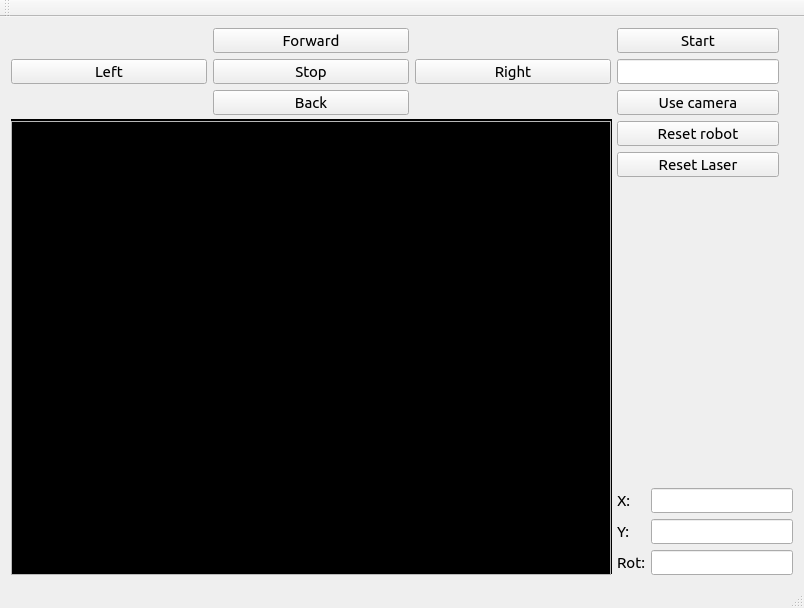
\includegraphics[width=0.5\textwidth]{img/oldUI.png}
	\end{center}
	\caption{Povodni výzor aplikácie a ovládanie robota.}\label{fig:oldUI}
\end{figure}

Tento dizajn ma niekoľko nedostatkov, ktoré sme mali za úlohu identifikovať a opraviť. Prvým problémom je,
že tlačidlá pre ovládanie robota sa nachádzajú nad zobrazovacou plochou. Toto umiestnenie je nevhodné, pretože
blokuje užívateľovi vo výhľade na robota. Druhým problémom je, že tlačidlá pre ovládanie robota sú príliš malé a
neprehľadné. Tretím problémom je, že tlačidlá pre ovládanie robota sú príliš blízko k sebe, čo môže spôsobiť
neúmyselné stlačenie viacerých tlačidiel naraz.

Ďalšie chybne prvky sa nachádzajú v samotnej funkcionalite aplikácie. Užívateľ sa vie pripojiť len na jedného robota
a to toho ktorý je v simulácii. Na pripojenie robota, ktorý je v reálnom svete je potrebné zmeniť IP adresu robota v kóde
a ten následne prekompilovať. Ak sa tlačidlo \textbf{Start} stlačí viackrát ako raz, tak aplikácia spadne. Tlačidlá
\textbf{Reset robot} a \textbf{Reset Laser} sú nepotrebné, pretože nemajú žiadnu funkcionalitu.

Následne poloha zobrazenia súradníc robota je nevhodná, pretože na ňu užívateľ nebude vidieť, keďže sú tlačidla na
ovládanie robota lokalizované nad obrazovkou zobrazujúcou dáta z lidaru alebo kamery.

Nedostatky tejto aplikácie sú ďalej len samotná implementácia zobrazenia dát z lidaru a kamery. Tieto dáta nie sú
spracované na vzájomné prepojenie.

\subsection{Nový dizajn}

Na základe identifikovaných problémov sme navrhli nový dizajn aplikácie. Tento dizajn je zobrazený na obrázkoch
\ref{fig:newUI}. Na obrázku \ref{fig:newUI} a je zobrazený základný dizajn aplikácie. Tento dizajn sa dá zmeniť cez
nastavenia \textit{Settings > Change style sheet}. Tlačidlá pre ovládanie robota boli v základnej verzii vymazane.
Robot sa ovláda pomocou klávesnice. A to klávesami W, A, S, D alebo šípkami. Pre zastavenie robota je potrebne stlačiť
klávesu R. Tato klávesa bola zvolená preto, aby sa zabránilo nežiadanému tlačeniu klávesy a tým zastavením robota.
Ďalej bol pridaný prvok na zmenu IP adresy robota.

\begin{figure}[!htbp]
	\centering

	\begin{subfigure}{0.49\textwidth}
		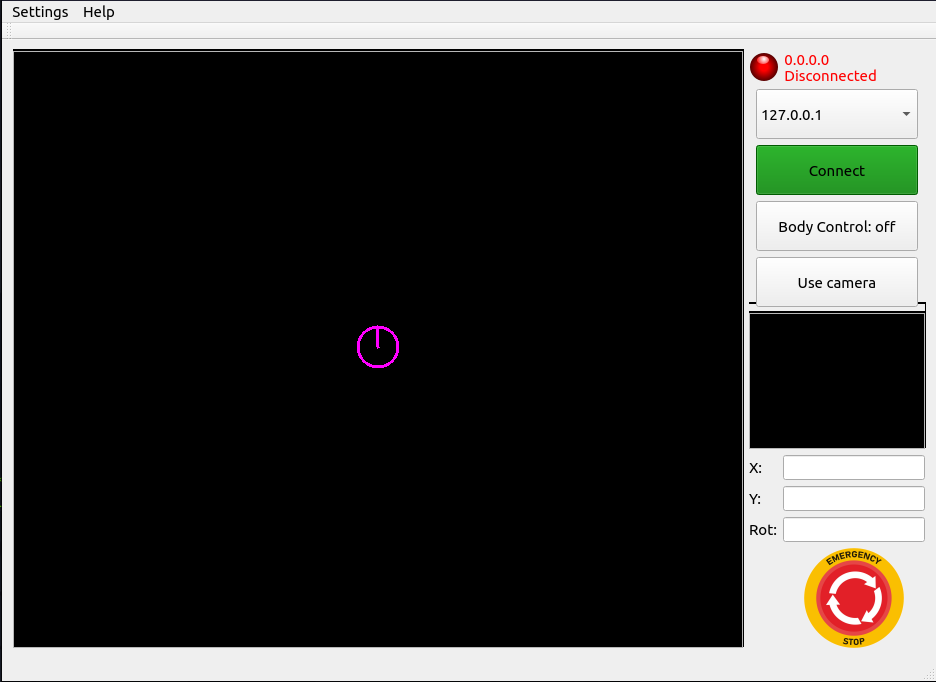
\includegraphics[width=\textwidth]{img/default-app.png}
	\end{subfigure}
	\hfill
	\begin{subfigure}{0.49\textwidth}
		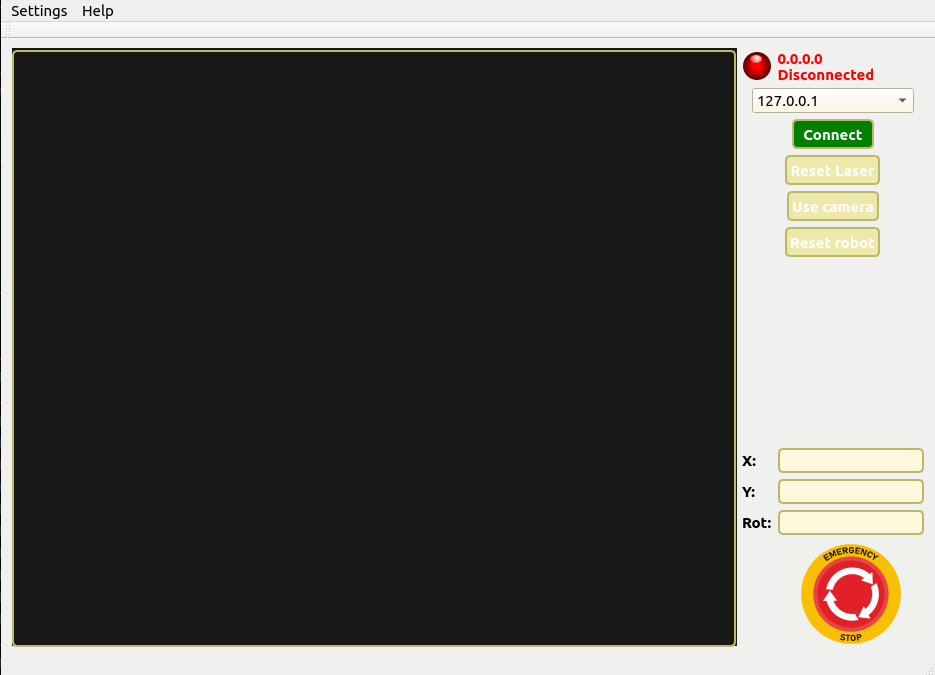
\includegraphics[width=\textwidth]{img/coffee-app.png}
	\end{subfigure}

	\vspace{\baselineskip}

	\begin{subfigure}{0.49\textwidth}
		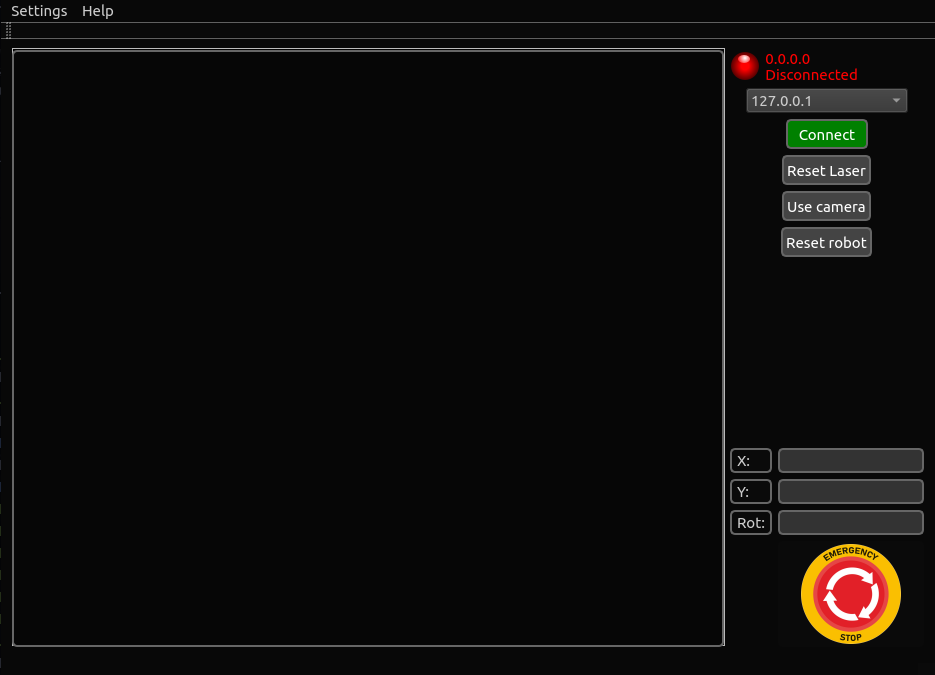
\includegraphics[width=\textwidth]{img/mocha-app.png}
	\end{subfigure}
	\caption{ Nove dizajny aplikácie zobrazujú základný (a), kávový (b) a mokka (c) mód.}
	\label{fig:newUI}
\end{figure}

Ako ďalšie prvky bol pridaný identifikátor stavu robota, ktorý zobrazuje či je robot pripojený, odpojený alebo v
núdzovom zastavení. Tieto stavy sú zobrazené na obrázkoch \ref{fig:led}

\begin{figure}[!htbp]
	\begin{subfigure}{0.3\textwidth}
		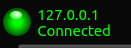
\includegraphics[width=\textwidth]{img/led-connected.png}
	\end{subfigure}
	\hfill
	\begin{subfigure}{0.3\textwidth}
		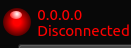
\includegraphics[width=\textwidth]{img/led-disconnected.png}
	\end{subfigure}
	\hfill
	\begin{subfigure}{0.3\textwidth}
		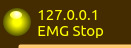
\includegraphics[width=\textwidth]{img/led-emg-stop.png}
	\end{subfigure}
	\caption{ Ledka zobrazujúca stav pripojenia k robotu (a), odpojenia od robota (b) a núdzového zastavenia (c).}
	\label{fig:led}
\end{figure}

Ďalší zmenený prvok je farebné zobrazenie tlačidla pripojenia a odpojenia robota. Keďže sú červena a zelená zlé farby na
kombináciu, bola zvolená aj zmena textu zobrazeného na tlačidle. Pri pripojení robota je zobrazený text \textbf{Connect}
a pri odpojení robota je zobrazený text \textbf{Disconnect}.

Taktiež bolo pridané softvérové tlačidlo pre núdzové zastavenie robota. Toto tlačidlo podľa normy HMI musí byť
umiestnene na viditeľnom mieste a musí byť veľké. Taktiež nemôže byť softvérové ale inú možnosť sme v tomto prípade
nemali (a taktiež to bolo v zadaní).

Pri stlačení tohto núdzového tlačidla sa zablokujú všetky vstupy z tlačidiel, klávesnice, a kamery. Jedinými
povolenými funkciami sú prepnutie medzi kamerou a lidarom a zrušenie núdzového stavu. Zobrazenie núdzového zastavenia
je zobrazený na obrázku \ref{fig:emergency}

\begin{figure}[!htbp]
	\begin{center}
		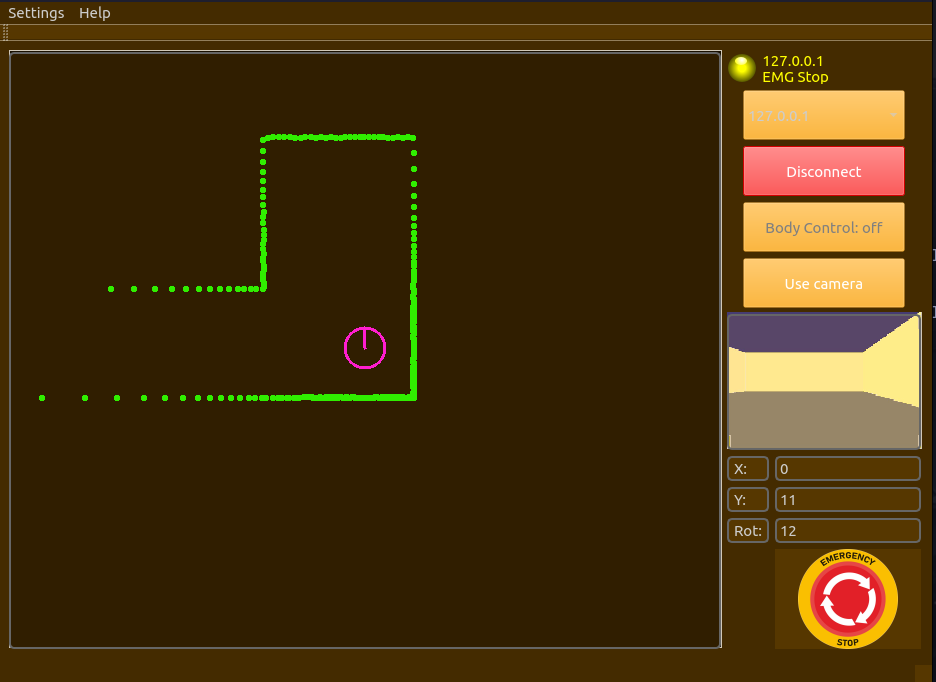
\includegraphics[width=0.95\textwidth]{img/app-emg-stop.png}
	\end{center}
	\caption{}\label{fig:emergency}
\end{figure}

Na obrázku \ref{fig:emergency} je zobrazené už aj zobrazenie dát z lidaru. Taktiež môžeme jednoznačne identifikovať
nezablokované tlačidla.

Ak by užívateľ používal túto aplikáciu na dotykovom displeji a chcel by ovláda robot pomocou tlačidiel, tak si môže
zobraziť tlačidlá pre ovládanie robota. Tieto tlačidla sú zobrazené na obrázku \ref{fig:touch}

\begin{figure}[!htbp]
	\begin{subfigure}{0.49\textwidth}
		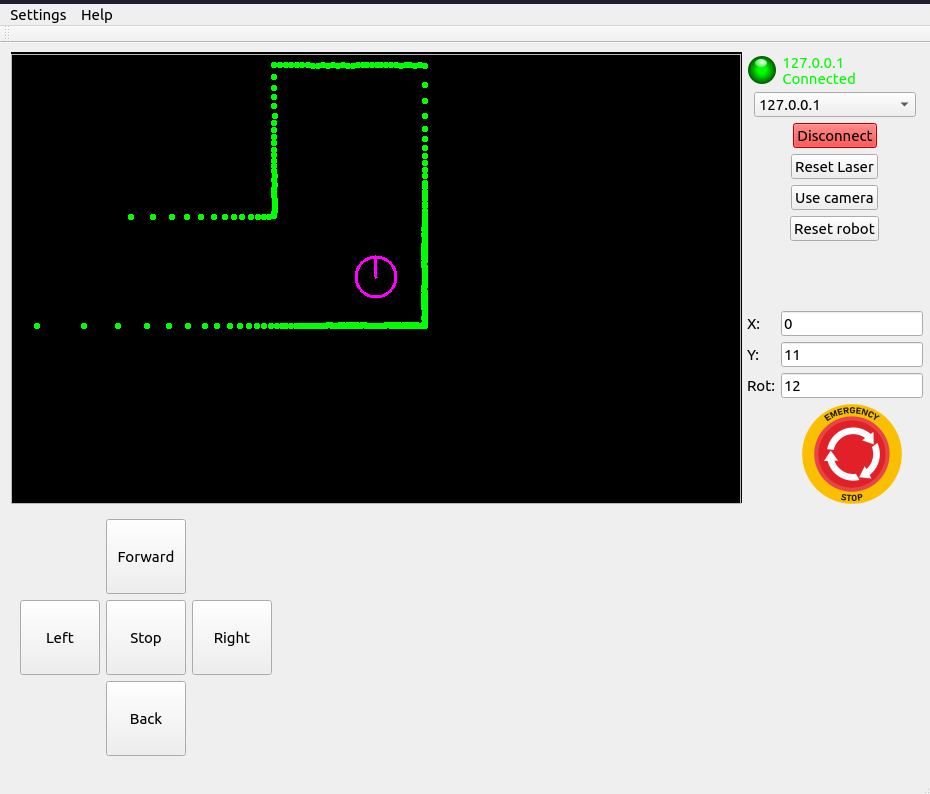
\includegraphics[width=\textwidth]{img/left-hand.png}
	\end{subfigure}
	\hfill
	\begin{subfigure}{0.49\textwidth}
		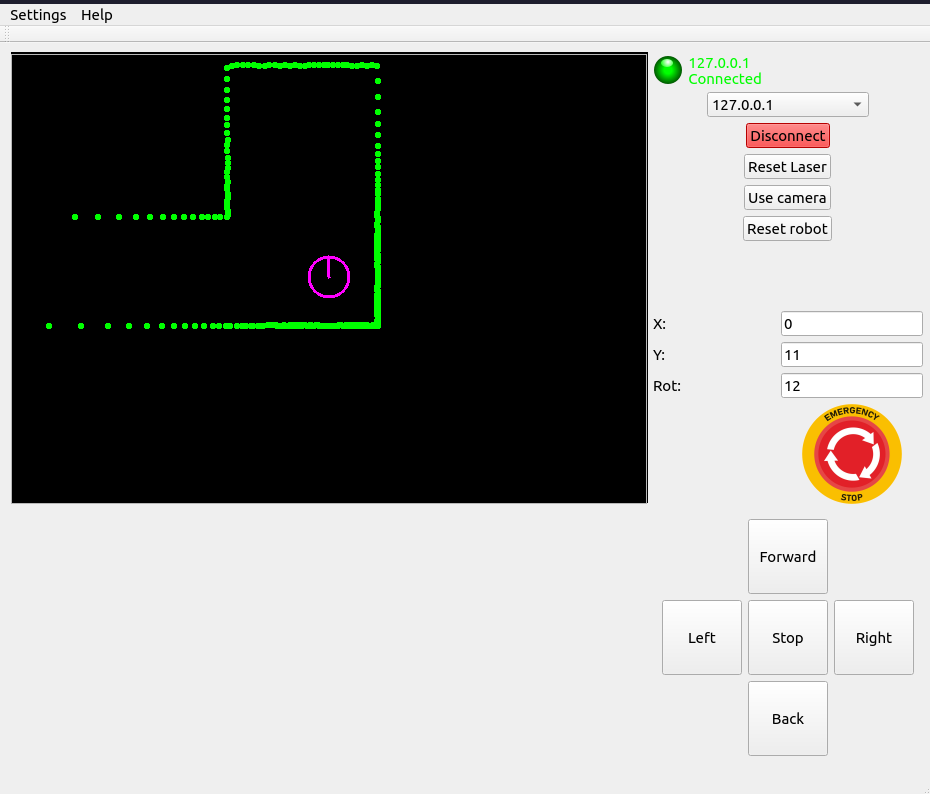
\includegraphics[width=\textwidth]{img/right-hand.png}
	\end{subfigure}
	\caption{ Dynamické zobrazenie tlačidiel pre ovládanie robota na dotykovom displeji. }
	\label{fig:touch}
\end{figure}

Ako vidine na obrázku \ref{fig:touch} tak sa tlačidla pre ovládanie robota zobrazujú len vtedy keď je v nastavení
zvolený mód s tlačidlami. Taktiež si užívateľ môže zvoliť, či chce mať tlačidlá na ľavej alebo pravej strane obrazovky.
Tieto tlačidla sú dostatočne veľké na to, aby ich užívateľ mohol ovládať aj na dotykovom displeji.

Pre jednoduchosť používania aplikácie a plochej krivke učenia sme pridali možnosť zobrazenia pomoci.
Tato pomoc je zobrazená na obrázku \ref{fig:help}. V tejto nápovede sme zvýraznili tie najdôležitejšie prvky,
aby si ich užívateľ vedel nájsť a vedel ich použivať v čo najkratšom čase.

\begin{figure}[!htbp]
	\begin{center}
		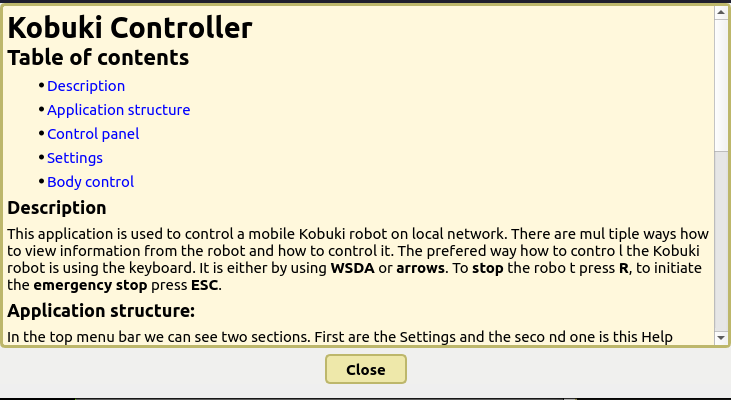
\includegraphics[width=0.95\textwidth]{img/help.png}
	\end{center}
	\caption{Pomoc pre užívateľa na zorientovanie sa v používaní aplikácie.}
	\label{fig:help}
\end{figure}

\section{Lidar Kamera fúzia}

\subsection{Problematika}
V tejto úlohe bolo potrebné vizualizovať na kamere dáta z lidaru, primárne tie ktoré niesu viditeľne kamerou, aby sme upozornili
operátora na možne kolízie a prekážky ktoré sa nachádzajú v pracovnom prostredí robota. Taktiež sme implementovali parkovaciu
kameru, ktorá sa zapne pri cúvaní s robotom, následne pri zmene smeru dopredu sa opäť zapne pôvodné okno, ktoré mal používateľ
zapnuté.

\subsection{Riešenie}

Robota sme si rozdelili na 8 častí a z nich sme následné spracovali dáta pre vizualizáciu. Robota delíme na prednú/zadnú časť
pravú/ľavú časť po 40 stupňov a pomedzi ne sú ďalšie 50 stupňov sektory, ktoré nám poskytujú ďalšie informácie o predmetoch
v okolí robota. Taktiež v HMI je implementovaný detektor kolízii. Parkovacia kamera vykresľuje primárne body za robotom,
ale ponecháva operátorovy informáciu aj o prekážkach pred robotom.

\subsection{Kamerová časť}

Detegovali sme prekážky ktoré sa nachádzajú už 80cm od robota, a ak sa predmet nachádzal bližšie než 50cm od robota, zvýšili
sme úroveň alarmu. Na kamere sa nevykresľujú dáta nachádzajúce sa priamo za robotom, ale zvýrazňujeme 7 sektorov v okolí robota.

Alarm výzera následovne:
\begin{figure}[!htbp]
	\begin{center}
		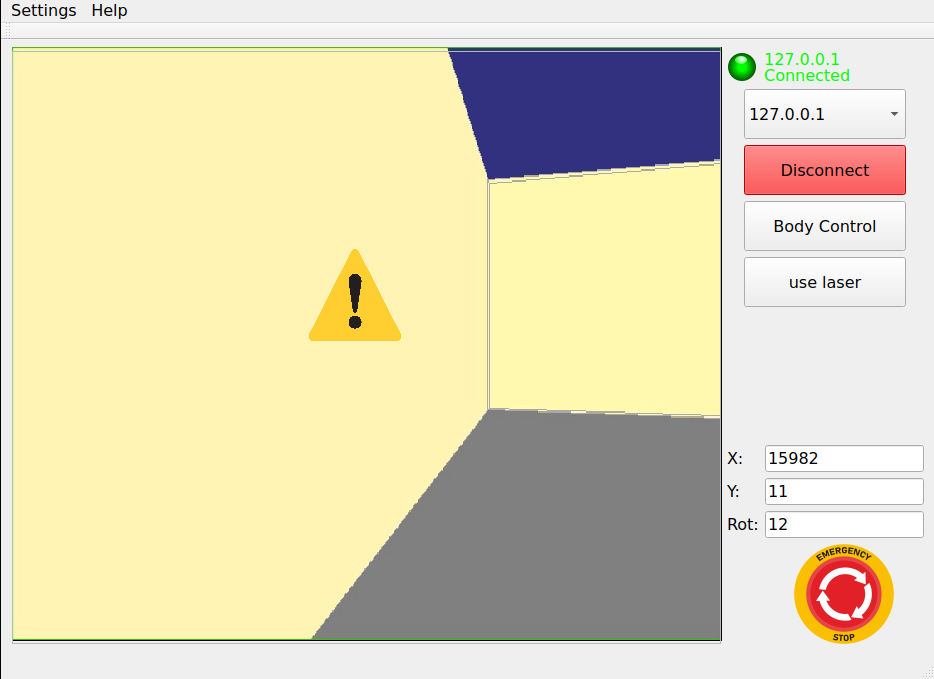
\includegraphics[width=0.95\textwidth]{img/alarm-all.png}
	\end{center}
	\caption{Alarmy použite na upozornenie operátora o objektoch v blízkosti robota}
	\label{fig:alarm}
\end{figure}

\subsection{Parkovacia kamera}

Pri zmene smere robota na chod vzad, sa automaticky zapne parkovacia kamera, na ktorej sa zafarbujú predmety ležiace za robotom.
Body postupne menia farbu z bezpečnej zelenej cez žltú na červenú farbu.

\begin{figure}[!htbp]
	\begin{center}
		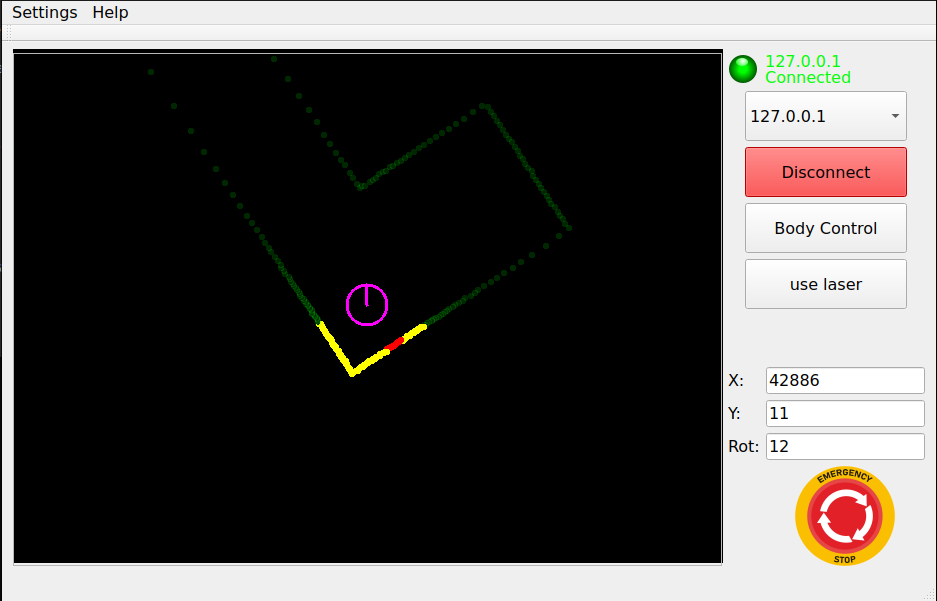
\includegraphics[width=0.95\textwidth]{img/parking_camera.png}
	\end{center}
	\caption{Parkovací asistent}
	\label{fig:parking}
\end{figure}

\section{Ovládanie gestami}

Ovládač reaguje na operátorove zápästie a lakeť pravej aj ľavej ruky. Pohyb je v prirodzenom pracovnom priestore kĺbov ruky.
S ľavou rukou sa nastavuje rýchlosť v pred aj vzad od 300 po -300 mm/s, zväčšením uhla medzi lakťom a zápästím sa rýchlosť pridáva a naopak.
Pravou rukou sa nastavuje rotačná rýchlosť rovnakým spôsobom ako pri rýchlosti, stým že rozmedzie je od -45 stupňov až 45 stupňov za sekundu.
Týmto typom ovládania je možne robotovi posielať tri typy rýchlosti.

\begin{figure}[!htbp]
	\begin{center}
		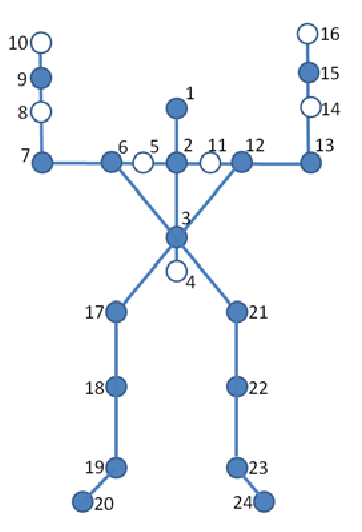
\includegraphics[width=0.35\textwidth]{img/skeleton.png}
	\end{center}
	\caption{Kĺby ľudského tela}
	\label{fig:skeleton}
\end{figure}

\newpage

Na \ref{fig:skeleton} sú znázornené kĺby ktoré sa na ľudskom tele detegujú. My sa zaoberáme kĺbom 7 voči 9 a 13 voči 15, kde obe ruky
sa sklápajú do vnútra. Nulové rýchlosti sú pri 45 stupňovom uhle.

Aby mal uzivatel aj spatnu vazbu o tom, ako aplikacia vnima natocenia jeho ruk, tak si moze pridat zobrazenie relativnej
hodnoty. Toto zobrazenie vidime na \ref{fig:progres-bars}.

\begin{figure}[!htbp]
	\centering

	\begin{subfigure}{0.49\textwidth}
		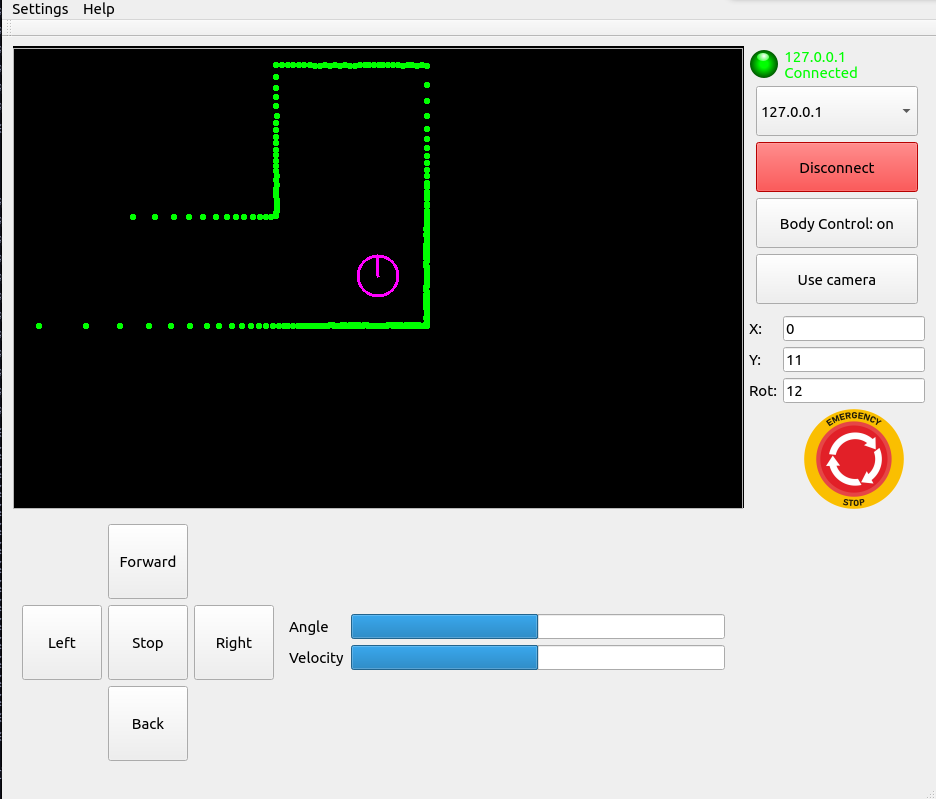
\includegraphics[width=\textwidth]{img/left-hand-body-control.png}
	\end{subfigure}
	\hfill
	\begin{subfigure}{0.49\textwidth}
		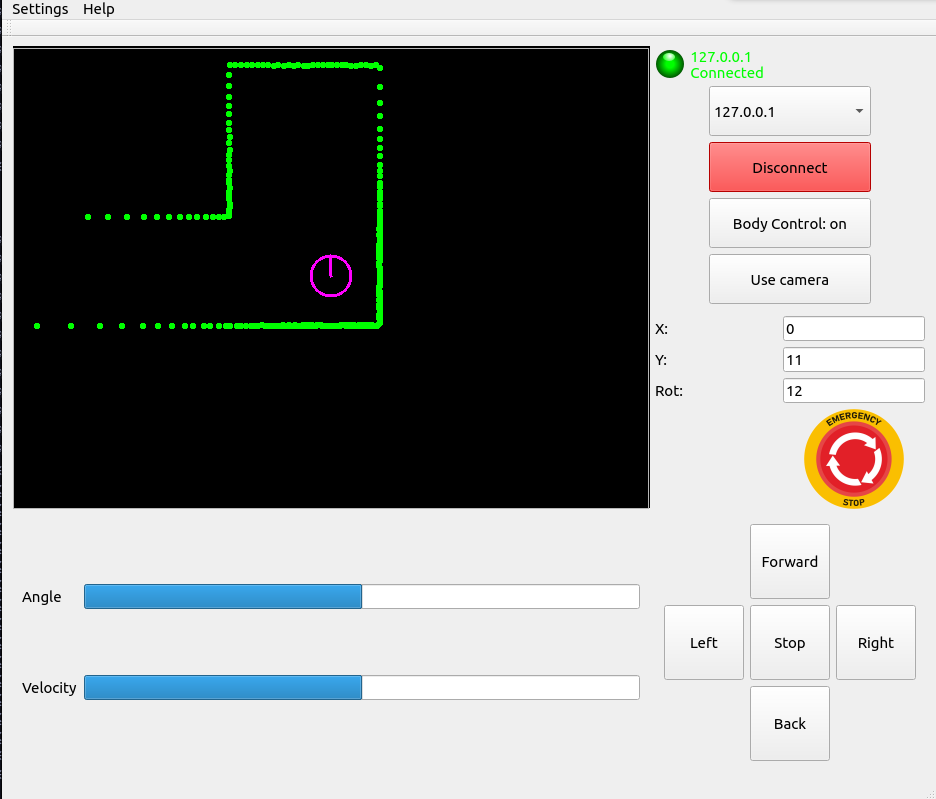
\includegraphics[width=\textwidth]{img/right-hand-body-control.png}
	\end{subfigure}

	\vspace{\baselineskip}

	\begin{subfigure}{0.49\textwidth}
		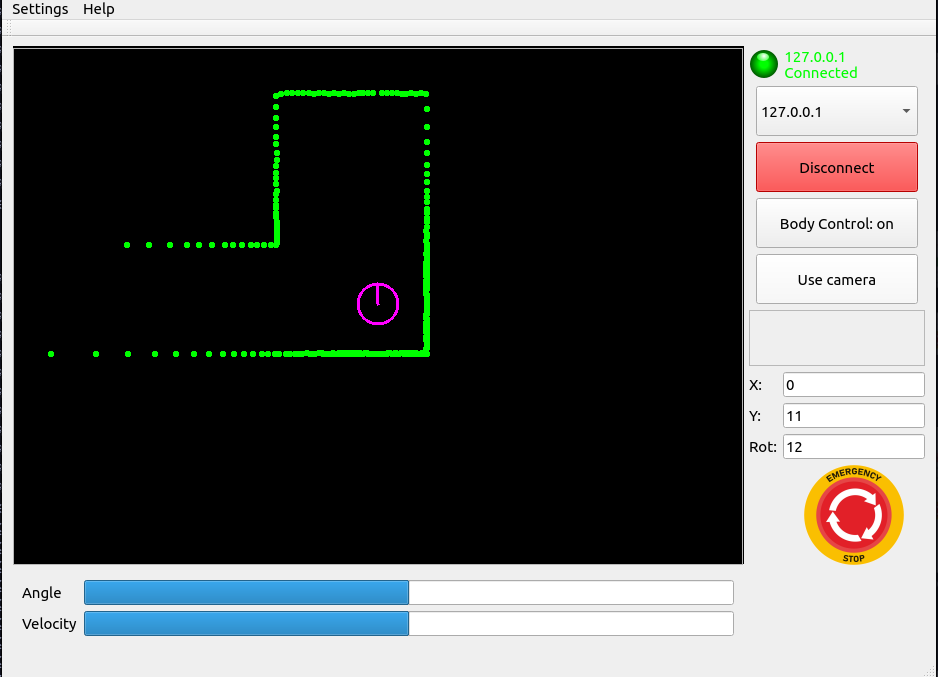
\includegraphics[width=\textwidth]{img/body-control.png}
	\end{subfigure}

	\caption{ Relativne zobrazenie polohy ruk na ovladanie robota. }
	\label{fig:progres-bars}
\end{figure}

Zaroven, ako si mozeme vsimnut, tak maly frame, krory sme mali na pravo od hlavnej zobrazujucej plochy nam zanikol.
Stalo sa to z dovodu, ze sme nemali dostatok miesta na jeho vykreslenie. Preto, aby sme neposkytovali necitatelne
inforamcie, tak sme sa rozhodli tento frame odstranit.

